\documentclass[review,fleqn]{elsarticle}
\usepackage{amsmath}
\usepackage{lineno,hyperref}
\usepackage[left=2cm, right=2cm, top=3cm, bottom=3cm]{geometry}
\usepackage{booktabs}
\usepackage{makecell}
\usepackage{tabularx}
\usepackage{amssymb}
\usepackage{array,caption,threeparttable}
\usepackage[font=small,labelfont=bf,labelsep=none]{caption}
\usepackage{graphicx}
\usepackage{epstopdf}
\usepackage{tikz}
\usepackage{verbatim}
\usepackage{cleveref}
\usepackage{hhline}

\hypersetup{
    colorlinks=true, % 允许超链接使用颜色
    linkcolor=blue,  % 图片引用链接颜色
}

\usetikzlibrary{matrix, positioning}
\modulolinenumbers[5]

\crefname{figure}{Fig.}{Figs.}
\crefname{table}{Table}{Table}
\newcommand{\figref}[1]{\hyperref[#1]{Fig.~\ref*{#1}}}
\newcommand{\tabref}[1]{\hyperref[#1]{Table~\ref*{#1}}}
\journal{Journal of \LaTeX\ Templates}

%%%%%%%%%%%%%%%%%%%%%%%
%% Elsevier bibliography styles
%%%%%%%%%%%%%%%%%%%%%%%
%% To change the style, put a % in front of the second line of the current style and
%% remove the % from the second line of the style you would like to use.
%%%%%%%%%%%%%%%%%%%%%%%

%% Numbered
%\bibliographystyle{model1-num-names}

%% Numbered without titles
%\bibliographystyle{model1a-num-names}

%% Harvard
%\bibliographystyle{model2-names.bst}\biboptions{authoryear}

%% Vancouver numbered
%\usepackage{numcompress}\bibliographystyle{model3-num-names}

%% Vancouver name/year
%\usepackage{numcompress}\bibliographystyle{model4-names}\biboptions{authoryear}

%% APA style
%\bibliographystyle{model5-names}\biboptions{authoryear}

%% AMA style
%\usepackage{numcompress}\bibliographystyle{model6-num-names}

%% `Elsevier LaTeX' style
\bibliographystyle{elsarticle-num}
%%%%%%%%%%%%%%%%%%%%%%%


\captionsetup[table]{
labelsep=newline,
singlelinecheck=false,
}
\captionsetup[figure]{name={Fig.},labelsep=period}
\begin{document}

\begin{frontmatter}

\title{Elsevier \LaTeX\ template\tnoteref{mytitlenote}}
\tnotetext[mytitlenote]{Fully documented templates are available in the elsarticle package on \href{http://www.ctan.org/tex-archive/macros/latex/contrib/elsarticle}{CTAN}.}

%% Group authors per affiliation:
\author{Elsevier\fnref{myfootnote}}
\address{Radarweg 29, Amsterdam}
\fntext[myfootnote]{Since 1880.}

%% or include affiliations in footnotes:
\author[mymainaddress,mysecondaryaddress]{Elsevier Inc}
\ead[url]{www.elsevier.com}

\author[mysecondaryaddress]{Global Customer Service\corref{mycorrespondingauthor}}
\cortext[mycorrespondingauthor]{Corresponding author}
\ead{support@elsevier.com}

\address[mymainaddress]{1600 John F Kennedy Boulevard, Philadelphia}
\address[mysecondaryaddress]{360 Park Avenue South, New York}

\begin{abstract}
This template helps you to create a properly formatted \LaTeX\ manuscript.
\end{abstract}

\begin{keyword}
\texttt{elsarticle.cls}\sep \LaTeX\sep Elsevier \sep template
\MSC[2010] 00-01\sep  99-00
\end{keyword}

\end{frontmatter}

\linenumbers

\section{The Elsevier article class}

\paragraph{Installation} If the document class \emph{elsarticle} is not available on your computer, you can download and install the system package \emph{texlive-publishers} (Linux) or install the \LaTeX\ package \emph{elsarticle} using the package manager of your \TeX\ installation, which is typically \TeX\ Live or Mik\TeX.

\paragraph{Usage} Once the package is properly installed, you can use the document class \emph{elsarticle} to create a manuscript. Please make sure that your manuscript follows the guidelines in the Guide for Authors of the relevant journal. It is not necessary to typeset your manuscript in exactly the same way as an article, unless you are submitting to a camera-ready copy (CRC) journal.

\paragraph{Functionality} The Elsevier article class is based on the standard article class and supports almost all of the functionality of that class. In addition, it features commands and options to format the
\begin{itemize}
\item document style
\item baselineskip
\item front matter
\item keywords and MSC codes
\item theorems, definitions and proofs
\item lables of enumerations
\item citation style and labeling.
\end{itemize}

\section{Description of RKC method }
\subsection{Classic one-step RKC methons}
Let $y_n$ represent the approximation to the exact solution $y(n)$ at time $t=t_n$ and $h=t_{n+1}-t_n$ 
is the time step size. For the ODE system(1),the formulas of one-step RKC method with s stage can be defined as 
\begin{equation}
 \begin{aligned}
    &K_{0}=y_{n}, \\
    &K_{1}=y_{n}+\tilde{u}_{1}hF_{0}, \\
    &K_{j}=u_{j}K_{j-1}+v_{j}K_{j-2}+(1-u_{j}-v_{j})K_{0}+\tilde{u}_{j}hF_{j-1}+\tilde{\gamma}_{j}hF_{0},\quad j\geq2, \\
    &y_{n+1}=K_{s},\quad n=0,1,\ldots,N-1, 
 \end{aligned}
 \label{eq:RKC2}
\end{equation}

where \(F_j = f(t_n + c_jh, K_j)\),and $y_0=y(t_0)$, the coefficients \(u_j, v_j, \tilde{u}_j, \tilde{v}_j, \tilde{\gamma}_j \in R \),
 $c_j$ has the following recursive format,
\begin{equation}
 \begin{aligned}
    &c_0=0,c_1=+\tilde{u_1},\\
    &c_j = u_j c_{j-1} + v_j c_{j-2} + \tilde{u}_j + \tilde{\gamma}_j, \quad 2 \leq j \leq s. 
 \end{aligned}
\end{equation}

Based on [],if the correlation coefficients satisfy the following conditions, 
then the RKC method \eqref{eq:RKC2} has second-order accuracy
\begin{equation}
 \begin{aligned}
    &\tilde{u}_{1} =b_{1} ,\quad \omega_{1}=\frac{T_{s}^{\prime}\quad(\omega_{0})}{T_{s}^{\prime\prime}(\omega_{0})}, \quad  \omega_{0}=1+\frac{\eta}{s^{2}}, \quad b_{0}=b_{1}=b_{2}, \\
    &u_{j} =2\omega_{0}\frac{b_{j}}{b_{j-1}},\quad v_{j}=-\frac{b_{j}}{b_{j-2}},\quad\tilde{u}_{j}=2\omega_{1}\frac{b_{j}}{b_{j-1}},  \\
    &\tilde{\gamma}_{j} =-\big(1-b_{j-1}T_{j-1}(\omega_{0})\big)\tilde{u}_{j},\quad b_{j}=\frac{T_{j}^{\prime\prime}(\omega_{0})}{\big(T_{j}^{\prime}(\omega_{0})\big)^{2}},\quad2\leq j\leq s, 
 \end{aligned}
 \label{eq:RKC_coefficient}
\end{equation}

Here, $\eta \geq 0$ is a small free damping parameter, and changing the value of $\eta$ typically alters the shape of the stability region,
for \eqref{eq:RKC2}, $\eta = \frac{2}{13}$ in \eqref{eq:RKC} is an appropriate value to use.

Apply the second-order RKC method \eqref{eq:RKC2} to the test problem $y'(t)=\lambda y(t),\quad \lambda \in \mathbb{C}$, and the expression for the second-order consistent stability function is as follows:
\begin{align}
    P_s(z)=1-b_sT_s(\omega_0)+b_sT_s(\omega_0+\omega_1z)
\end{align}

where $a_{j}=1-b_{j}T_{j}(\omega_{0}).$

The stabilisation domain of the RKC method is usually a narrow region around the negative real axis, whose length is proportional to $s^2$
,for the second-order method described above, the real stabilisation interval is $[-0.65s^2,0]$ , and the optimal parameters can be chosen so that the length of the negative real-axis interval reaches approximately $0.81s^2$, as described in $[]$.

\subsection{The two-step RKC method}

The two-step RKC method  \eqref{eq:TRKC} was devised by B.P. Sommeijer et al [111]. in 2007, which has a similar formulation to the multi-step method, assuming that $y_{n-1},y_{n}$ are the numerical solutions obtained from the two-step RKC computed in times $t_{n-1},t_{n}$
.It is represented by the formula:
\begin{align}
    y_{n+1}=\alpha_{-1}y_{n-1}+\alpha_{0}y_{n}+\alpha\tilde{y_{n+\theta}},
\label{eq:TRKC}
\end{align}

We initiate the process by employing the RKC formula \eqref{eq:RKC2} at $t = t_{n}$, commencing with an initial value of $y_{n}$ and a step size of $\theta h_{n}$. This step yields a result in a single iteration, denoted as $y_{n+\theta}$.
Subsequently, we calculate the new value $y_{n+1}$ using the two-step RKC formula \eqref{eq:TRKC}. This particular method, given that $y_{n-1}$ and $y_{n}$ are known, requires just one more storage unit compared to the one-step approach. However,
 it offers a notable advantage in terms of the $\omega_{1}$ parameter. Selecting an appropriate value for $\omega_{1}$ can significantly expand the extent of the stability domain, particularly around the negative real axis.
To establish an additional initial value, we perform one step using the one-step RKC method \eqref{eq:RKC2} at the beginning. From the second step onward, we transition to employing the two-step RKC method \eqref{eq:TRKC}.

The new parameters $\alpha_{-1}, \alpha_{0}, \alpha \in \mathbb{R} $ are used to control the convergence order of the two-step methods \eqref{eq:TRKC}. To be precise, we compute the Taylor expansion of $\tilde{y}_{n+\theta}$ and $y_{n-1}$.
\begin{align}
    &\tilde{y}_{n+\theta}=y_n+\theta\tau_ny_n^{\prime}+\frac12\theta^2\tau_n^2y_n^{\prime\prime}+\frac16c\theta^3\tau_n^3y_n^{\prime\prime\prime}+\mathcal{O}(\tau_n^4),\quad c=\frac{T_s^{\prime}(\omega_0)T_s^{\prime\prime\prime}(\omega_0)}{T_s^{\prime\prime}(\omega_0)^2},\\
    &{y}_{n-1}=y_n-\tau_{n-1}y^{\prime}+\frac12\tau_{n-1}^2y_n^{\prime\prime}-\frac16\tau_{n-1}^3y_n^{\prime\prime\prime}+\mathcal{O}(\tau_n^4)
 \end{align}

Comparison of these formulas with the Taylor expansion of the true solution, the two-step RKC method converges thrid order for linear problems $W^{\prime}=AW$if the conditions
\begin{equation}
 \begin{aligned}
 &\alpha_0 = 1 - \alpha_{-1} - \alpha_{\theta}, \quad \alpha_{\theta} = \frac{1 + r_n}{\theta(1 + \theta r_n)}, \quad \alpha_{-1} = \frac{r_n^2(1 - \theta)}{1 + \theta r_n},\\
 &(cr_{n})\theta^{2}+(1-r_{n})\theta-1=0,
 \end{aligned}
 \label{eq:TRKC_coefficient}
\end{equation}
where $r_n=\frac{\tau_n}{\tau_{n-1}}$ is the step ratio,equation \eqref{eq:TRKC_coefficient} always has two real roots for $\theta$,one of which is negative. Naturally, we require the positive root.
Notably, $s>3$ and $1<\theta<2$ are necessary conditions .If the parameters $\alpha_{-1}, \alpha_{0}, \alpha $ just satisfy the condition \eqref{eq:TRKC_coefficient}, then method \eqref{eq:TRKC} has second-order consistency for the nonlinear problem
We consider two-step methods with a constant step size that maintain third-order consistency. It is then $\theta = \frac{1}{c}$, insert $y_j=\zeta^j$ into \eqref{eq:TRKC}. This leads to the corresponding characteristic equation:

\begin{align}
\zeta^2 - (\alpha_0 + \alpha_\eta P_s(\theta z))\zeta - \alpha_{-1} = 0 
\label{eq:TRKCploy}
\end{align}

The stability regions are determined through numerical construction based on the root condition []. Let $\tilde{\beta(s)}$ donate the real stability boundary,similar to the one-step RKC method \eqref{eq:RKC2}, 
the value of the damping parameter $\varepsilon$ adjustment can also change the shape of the stabilization domain, and suitable values of $\varepsilon$ have been found. For more details, refer to [].



\section{The new two-step RKC formula}

Assume that $y_{n-1},y_n$ are the numerical solutions obtained from the new two-step RKC method \eqref{eq:NTRKC} at times $t_{n-1},t_n$, and $\tilde{y}_{n-1},\tilde{y}_n$ are obtained by applying a one-step method \eqref{eq:RKC2} to $y_{n-1},y_n$ with step sizes $\tau_{n-1}$ and $\tau_n$, respectively.
The new two-step method then determines the approximation $y_{n+1}$ at the future time level $t_{n+1}$ as follows:
\begin{align}
    y_{n+1} = \alpha_{-1}y_{n-1} + \tilde{\alpha}_{-1}\tilde{y}_{n-1} + \alpha_0y_n + \alpha\tilde{y}_n,
    \label{eq:NTRKC}
\end{align}

 By introducing new coefficients $\tilde{\alpha_{-1}}$ and enhancing the retention of results from previous one-step RKC calculations,
 the computational overhead remains almost unchanged when compared to the two-step RKC method. However, 
 the inclusion of $\tilde{\alpha_{-1}}$ grants us extra maneuverability for adjusting $\omega_{1}$. Consequently, the coefficients $\eta$, $\omega_{0}$, 
 and $\omega_{1}$  \eqref{eq:RKC_coefficient} in the NTRKC scheme exhibit slight deviations from those of the one-step RKC method. 
 In the context of NTRKC, the modulation of the damping parameter $\varepsilon$ and $\omega_{1}$ serves to shape the stabilizing domain. Higher values of $\varepsilon$ 
 and $\omega_{1}$ entail a trade-off between domain width and length, favoring a wider region at the expense of domain length. Conversely, lower values of $\varepsilon$ and $\omega_{1}$ 
 lead to a more elongated yet narrower stabilizing domain. Notably, NTRKC \eqref{eq:NTRKC} demonstrates superior stabilizing domain characteristics when compared to the two-step RKC method \eqref{eq:TRKC}, 
 yielding heightened numerical accuracy. In the subsequent section dedicated to stabilizing domain analysis, we will delve further into this topic, 
 providing insights and presenting two distinct sets of coefficients



\subsection{Convergence Analysis}
The parameters$ \alpha_{-1},\tilde{\alpha_{-1},\alpha_{0},\alpha} \in  \mathbb{R} $ are used to control the convergence order of the method \eqref{eq:NTRKC}.
Based on [1],Explict Runge-Kutta method \eqref{eq:RKC2} can be written in a tabular format

\begin{center}
\vspace{10pt} 
\begin{tabular}{c|c c c c c}

    
       0    &  &  &  &  &  \\
  
    $c_1$ & $a_{11}$ &  &  &  &  \\

    $c_2$ & $a_{21}$ & $a_{22}$ &  &  &  \\
 
    $\vdots$ & $\vdots$ & $\vdots$ & $\ddots$ &  &  \\
    
    $c_{s-1}$ & $a_{s-1,1}$ & $a_{s-1,2}$ &$\cdots$ & $a_{s-1,s-1}$ &   \\
    \hline
    $c_{s}$ & $a_{s,1}$ & $a_{s,2}$ &$\cdots$ & $a_{s,s-1}$ & $a_{s,s}$  \\
    
\end{tabular}
\vspace{10pt}
\end{center}
where the elements in the table are determined by \eqref{eq:RKC_coefficient}
\begin{equation}
    \begin{aligned}
       & A=\begin{bmatrix}
            &  &  &  & \\
            a_{11} &  &  & & \\
            a_{21} & a_{22} &  & & \\
            \vdots & \vdots & \ddots & & \\
            a_{s-1,1} & a_{s-1,2} & \cdots & a_{s-1,s-1}
        \end{bmatrix},
        b=\begin{bmatrix}
            a_{s,1} & a_{s,2}&\cdots & a_{s,s-1} & a_{s,s} 
        \end{bmatrix}\\
      & a_{11}=\tilde{u_1},\\
       & a_{j,j}=\tilde{u_{j}},\quad a_{j,1}=a_{j-1,1}u_{j}+a_{j-2,1}v_{j}+\tilde{v_j},\\
      &  a_{j,i}=a_{j-1,i}u_{j}+a_{j-2,i}v_{j},\quad 2 \le  j \le s, \quad 2 \le i  \le j-1 
    \end{aligned}
\end{equation}


 Let $y_{n-1},y_{n}$ denote approximations to $ y(t_n),y(t_{n-1})$,e is a column vector of s$\times$1 all its elements are equal to 1.Fixing the time step $\tau_{n}=\tau_{n-1}=\tau$,$\tilde{y_{n-1}}$ has the following estimator due to the change in $\omega_{1}$
 \begin{align}
     &A_1=\sum_{i=1}^{s}a_{s,i},\quad  A_2=b[Ae],\nonumber \\
     &A_3=b[Ae]\bullet[Ae],\quad A_4=bA[Ae],\nonumber \\
    &\tilde{y}_{n-1} = y_{n-1} + A_1\tau f_{n-1} + A_2\tau^2f'f_{n-1} + A_3\tau^3f'f'f_{n-1} + A_4\tau^3f''f^2_{n-1} + \mathcal{O}(\tau^4) 
     \label{eq:-y(n-1)}
\end{align}
where $f_{n-1}=f(y_{n-1})$,$ \tilde{y_{n-1}},\tilde{y_n}$ are both obtained by the method \eqref{eq:RKC2}, therefore $y_n$ has the same coefficients of the estimator.Considering $f_{n-1}$ as  function with respect to $\tau$,it is readily verified that 
\begin{align}
    f_{n-1} &= f_n + f_n'(y_{n-1} - y_n) + \frac{1}{2}f_n''(y_{n-1} - y_n)^2 + \mathcal{O}(\tau_n^4), \label{eq:f(n-1)} \\
    y_{n-1} &= y_n - \tau f_n + \frac{1}{2}\tau^2f_n'f_n - \frac{1}{6}\tau^3(f_n'f_n'f_n + f_n''f_n^2) + \mathcal{O}(\tau_n^4), \label{eq:y(n-1)}
\end{align}
insert \eqref{eq:f(n-1)} and \eqref{eq:y(n-1)} into \eqref{eq:-y(n-1)} we obtain
\begin{equation}
 \begin{aligned}
    \tilde{y}_{n-1} &= y_n + (A_1-1)\tau f_n + \left(\frac{1}{2}-A_1+A_2\right)\tau^2f_nf'_n  \\
    &\quad + \left(-\frac{1}{6}-\frac{A_2}{2}+A_3\right)\tau^3f'_nf'_nf_n \\
    &\quad + \left(-\frac{1}{6}+\frac{A_1}{2}-A_2+A_4\right)\tau^3f''_nf_n^2 + \mathcal{O}(\tau_n^4).
 \end{aligned}
\end{equation}
Let us denote $\tilde{A_1}=A_1-1$, $\tilde{A_2}=\frac{1}{2}-A_1+A_2$, $\tilde{A_3}=-1/6-(A_2/2)+A_3$, and $\tilde{A_4}=-1/6+(A_1/2)-A_2+A_4$. By comparing the corresponding coefficients in the expansions on both sides of \eqref{eq:NTRKC}, we can establish the linear third-order consistency condition for NTRKC:
\begin{equation}
  \begin{aligned}
    &\alpha _1+\alpha_2+\alpha_3+\alpha _4=1, \\
    &\alpha _1-\tilde{A_1}\alpha _2-\alpha _4A_1=-1, \\
    &\frac{\alpha _1}{2}+\tilde{A_2}\alpha_2+A_2\alpha _4=\frac{1}{2} ,\\
    &\frac{\alpha _1}{6}-\tilde{A_3}\alpha_3-A_3\alpha _4=-\frac{1}{6}   
  \end{aligned}
\end{equation}

It is possible to impose third-order consistency for the nonlinear problem  by defining $-\frac{1}{6}\alpha_1+\frac{1}{2}\tilde{A_4}\alpha_2+\frac{1}{2}A_4\alpha_4=\frac{1}{6}$,
,but for stability domain considerations here only the third order consistency condition is required and observe that the coefficients $\varepsilon_1=\frac{1}{6}+\frac{1}{6}\alpha_1-\frac{1}{2}\tilde{A_4}\alpha_2-\frac{1}{2}A_4\alpha_4$.
For example, for $s=10$, we have $\varepsilon_1=6.5\times10^{-6}$. This small number means that NTRKC is almost third-order for nonlinear problems. For comparison with two-step RKC(2.2.1),we can denote $\varepsilon_2$ as the coefficient of the fourth term 
of the two-step RKC \eqref{eq:TRKC} expansion subtracted by 1/6. It has $\varepsilon_2=0.07$ for $s=10$, which indicates that NTRKC will perform better than the two-step RKC in problems with strong nonlinear terms.

\tabref{table:1} presents a comparative analysis of $\varepsilon_1$ and $\varepsilon_2$ between the two-step RKC and NTERKC methods across a range of different stage number s. 
It becomes evident that, particularly at lower s stages, $\varepsilon_1$ is substantially smaller than $\varepsilon_2$. Moreover, as s increases, $\varepsilon_1$ exhibits only marginal changes, whereas $\varepsilon_1$ experiences a remarkable reduction. 
This observation underscores the superior convergence accuracy of NTERKC over the two-step RKC method, especially in the context of nonlinear problems. Notably,
 this performance advantage becomes more pronounced with higher levels of system rigidity





\begin{table}[!htbp]
    \centering
    \setlength{\abovecaptionskip}{0pt}
    \setlength{\belowcaptionskip}{10pt}
    \caption{Absolute values of $\varepsilon_1,\varepsilon_2$ for $s=5,7,9,11,13,50,100$}
    \label{table:1}
    \begin{tabularx}{\textwidth}{X *{8}{>{\centering\arraybackslash}X}}
      \toprule
      \multicolumn{1}{l}{s} & 5 & 7 & 9 & 11 & 13 & 50 & 100 \\
      \midrule
      $\varepsilon_1$ & $5.35\times10^{-6}$ & $2.1\times10^{-5}$ & $9.7\times10^{-6}$ & $4.4\times10^{-6}$ & $2.1\times10^{-6}$ & $3.6\times10^{-9}$ & $1.1\times10^{-10}$ \\
      $\varepsilon_2$ & 0.07 & 0.07 & 0.07&0.07 & 0.07 &0.07 &0.07 \\
      \bottomrule\addlinespace[1ex]
    \end{tabularx}
\end{table}
\subsection{Stability domains}
Since $\tilde{y_{n-1}},\tilde{y_n}$ are computed by the RKC method \eqref{eq:RKC2}, considering the stability domain with  constant step size, method \eqref{eq:NTRKC} leads to the characteristic equation $\varrho(\zeta)$
\begin{align}
    \zeta^2-(\alpha_0+\alpha P_s(z))\zeta-(\alpha_{-1}+\tilde{\alpha_{-1}}P_s(z))=0,\quad\quad\quad z\in C     
    \label{eq:NTRKCploy}
\end{align}
Based on root condition[44444],The method \eqref{eq:NTRKC} is called stable,if the roots of $\varrho(\zeta)$ \eqref{eq:NTRKCploy } lie on or within the unit circle,and the roots on the unit circle are simple.
Let $\beta(s)$ denote the real stability boundary,the key improvement of this method lies in the introduction of a new coefficient $\tilde{\alpha_{-1}}$ to obtain the ability to adjust $\omega_1$, which determines the size of $\beta_{s}$.
 The value range of $\omega_1$ is $frac{1+\omega_0}{cs^2},\quad c \in [0,0.65]$, and the corresponding real boundary is $\beta(s)\approx\frac{1+\omega _0}{\omega_1}\approx cs^2 $. The damping coefficient is also used to adjust the shape of the stabilisation domain. 
 Numerical experiments have proved that longer stable domains are more restrictive on damping coefficients usually, 
 small damping coefficients are needed, whereas for shorter stable domains larger damping coefficients can be chosen for wider widths, and here we have proposed two sets of schemes:
\begin{align}
    &\omega_1=\frac{1+\omega_0}{0.65 s^2},\quad \quad \varepsilon=0.05,\label{eq:long}\\
    &\omega_1=\frac{1+\omega_0}{0.45 s^2},\quad \quad \varepsilon=4,
    \label{eq:wide}
\end{align}
The first set \eqref{eq:long} has a narrow and long domain, while the second \eqref{eq:wide} has a shorter domain but with a significant increase in width.
\begin{figure*}[ht]
    \centering
    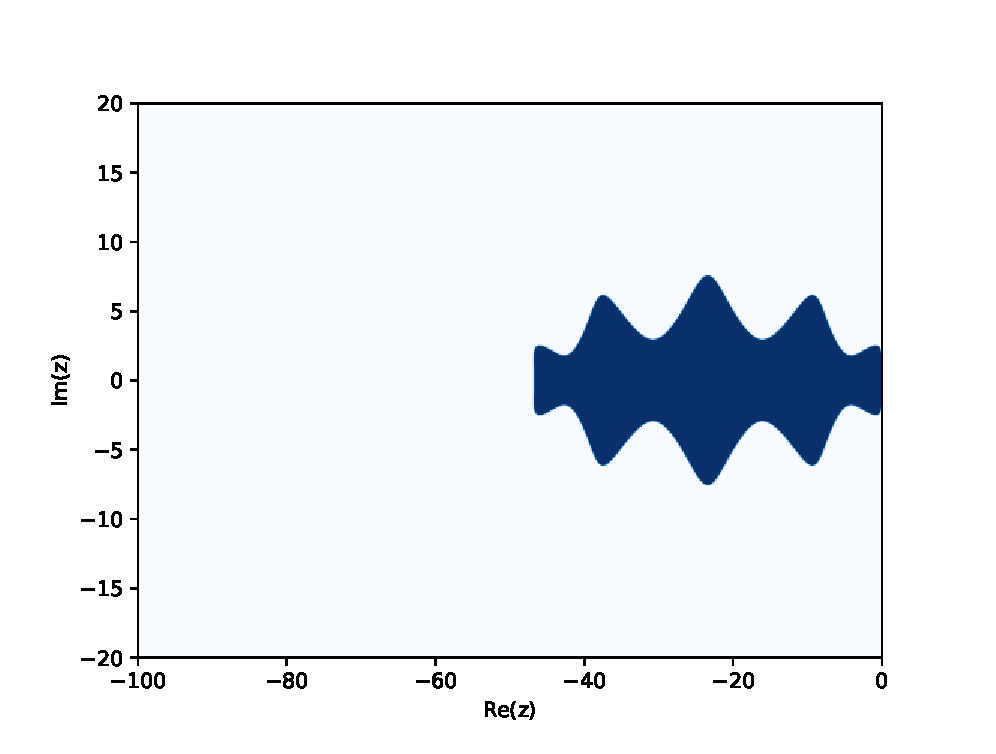
\includegraphics[width=0.3\linewidth]{stable_domians/twostepRKCs10.eps}
    \hfill
    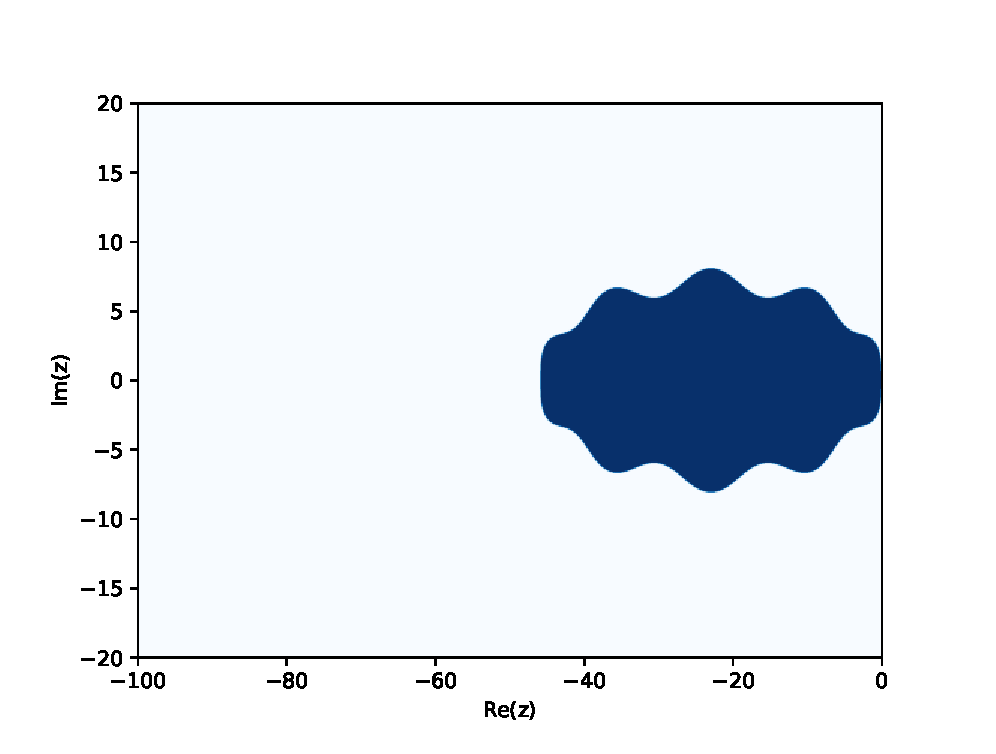
\includegraphics[width=0.3\linewidth]{stable_domians/NTRCKs10wide.eps}
    \hfill
    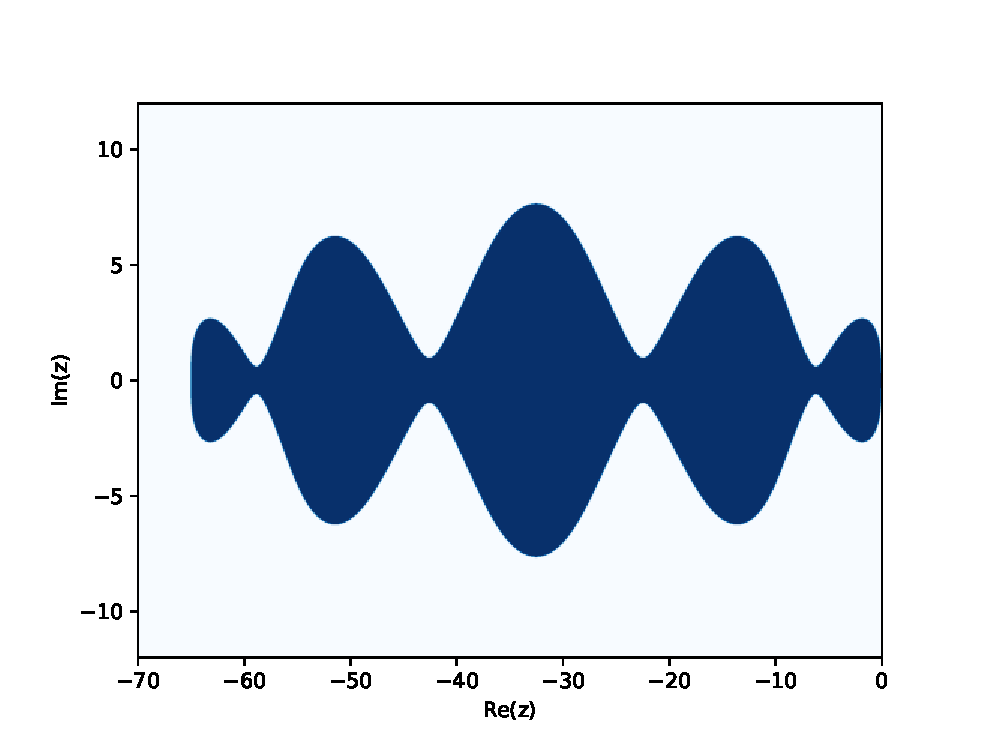
\includegraphics[width=0.3\linewidth]{stable_domians/NTRCKs10long.eps}
    \caption{ Stability domains of method (2.2.1) (left) , NTRKC  with $\varepsilon$ = 4,$\omega_1=\frac{1+\omega_0}{0.45s^2}$ (middle) and  NTRKC  with $\varepsilon$ = 0.05,$\omega_1=\frac{1+\omega_0}{0.65s^2}$ (right) for s=10.}
    \label{fig:1}
\end{figure*}
\begin{figure*}[ht]
    \centering
    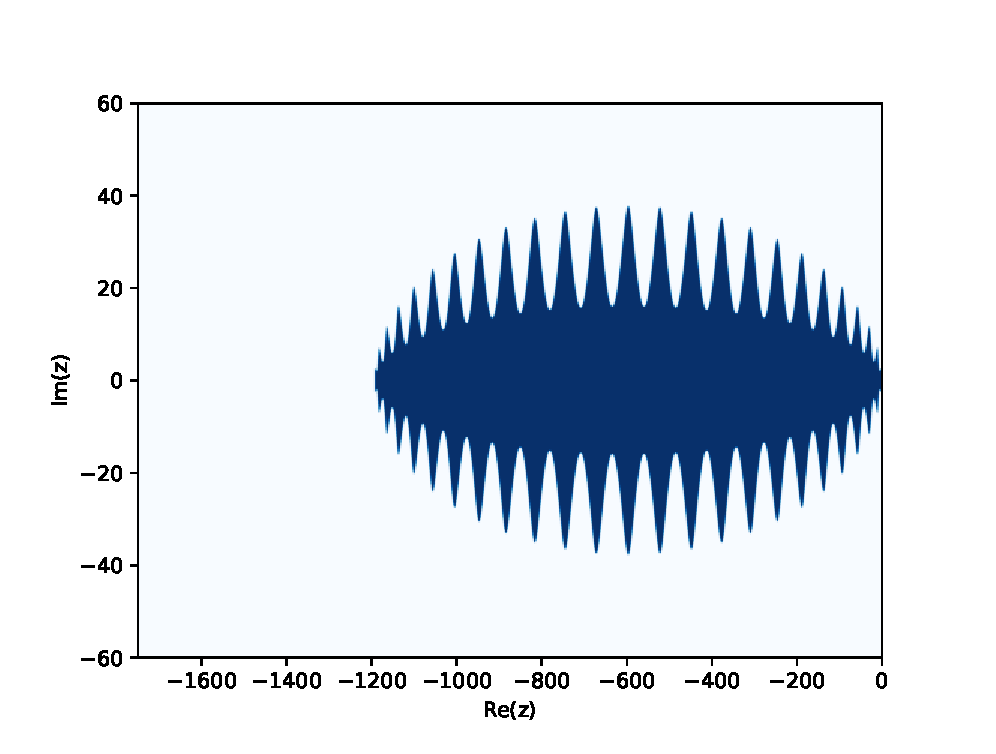
\includegraphics[width=0.3\linewidth]{stable_domians/twostepRKCs50.eps}
    \hfill
    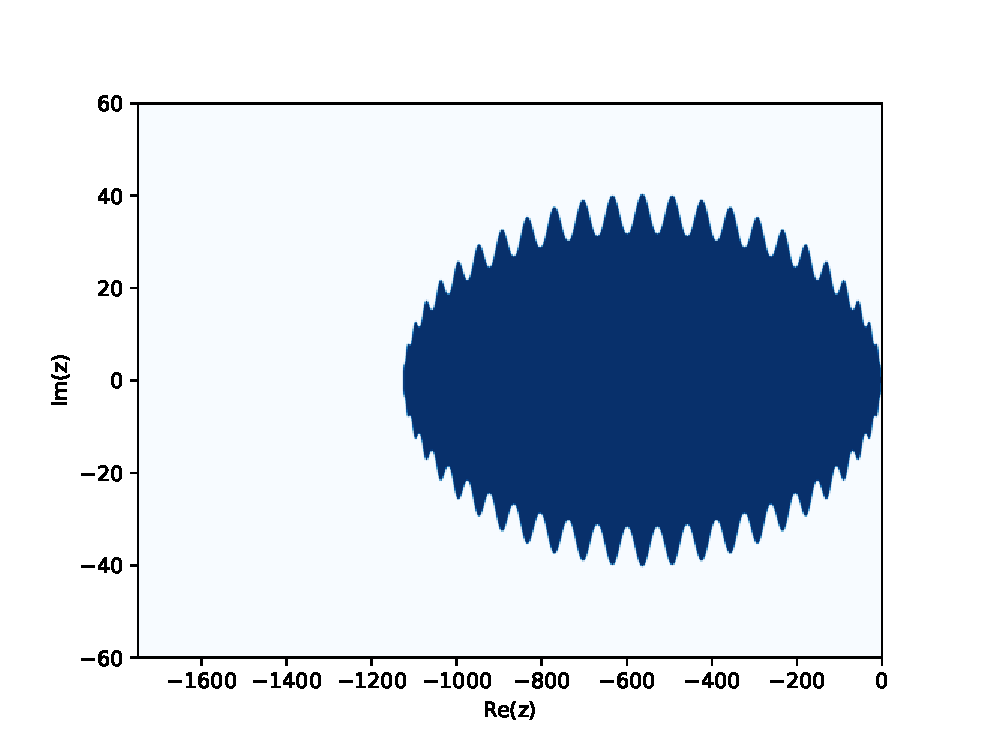
\includegraphics[width=0.3\linewidth]{stable_domians/NTRCKs50wide.eps}
    \hfill
    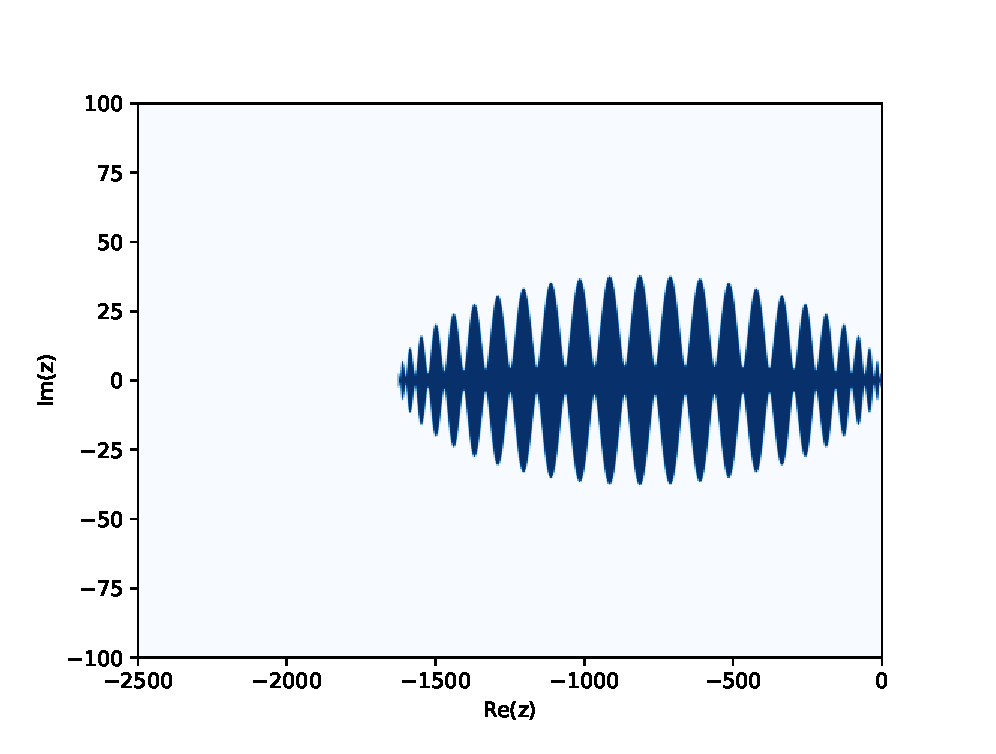
\includegraphics[width=0.3\linewidth]{stable_domians/NTRCKs50long.eps}
    \caption{ Stability domains of method (2.2.1) (left) , NTRKC  with $\varepsilon$ = 4,$\omega_1=\frac{1+\omega_0}{0.45s^2}$ (middle) and  NTRKC  with $\varepsilon$ = 0.05,$\omega_1=\frac{1+\omega_0}{0.65s^2}$ (right) for s=50}
    \label{fig:2}
\end{figure*}
\begin{figure*}[ht]
    \centering
    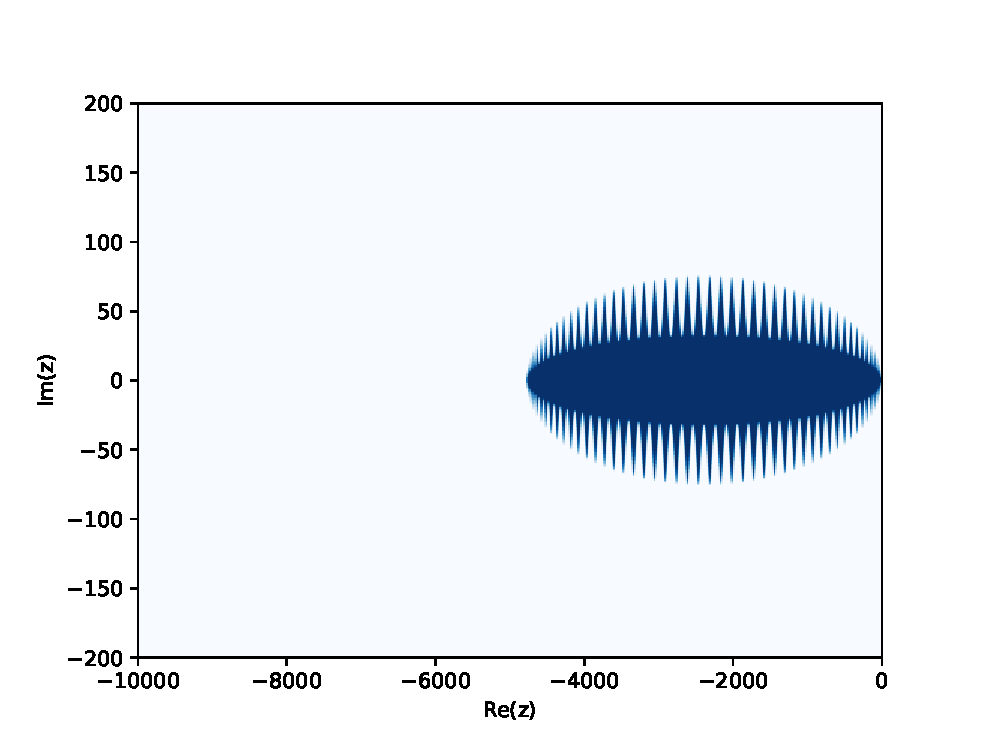
\includegraphics[width=0.3\linewidth]{stable_domians/twostepRKCs100.eps}
    \hfill
    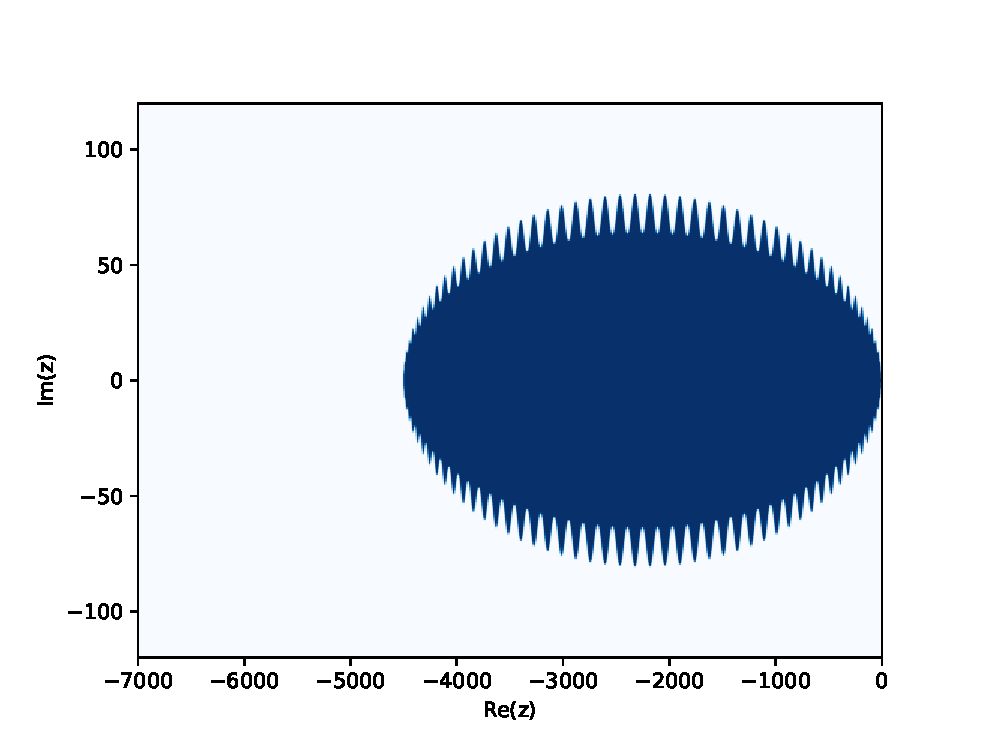
\includegraphics[width=0.3\linewidth]{stable_domians/NTRCKs100wide.eps}
    \hfill
    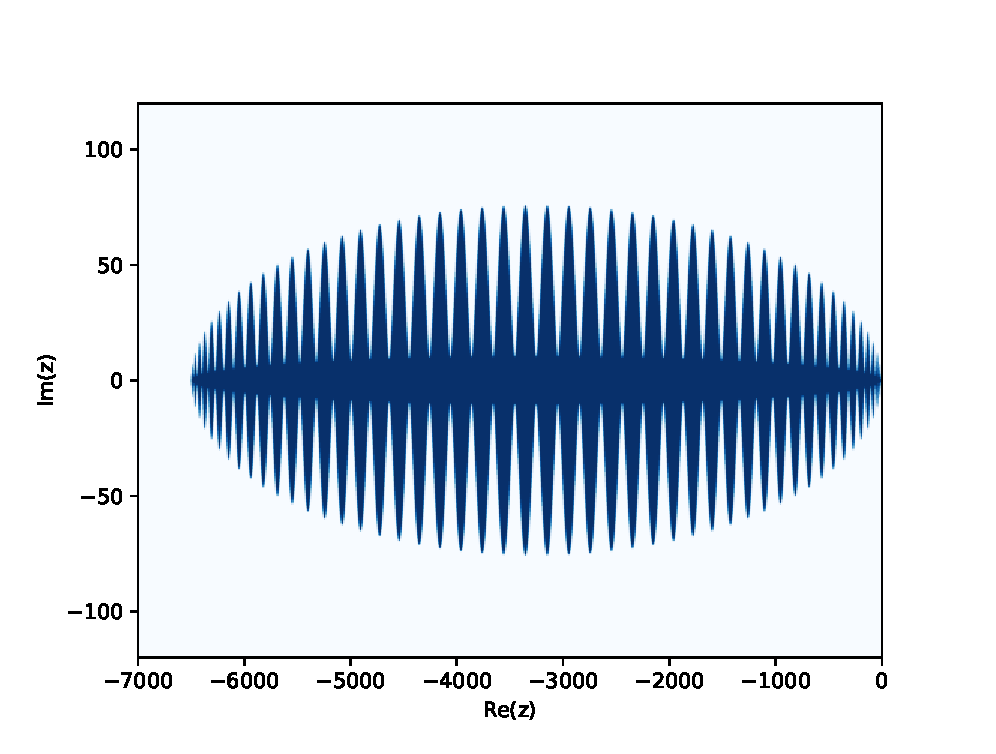
\includegraphics[width=0.3\linewidth]{stable_domians/NTRCKs100long.eps}
    \caption{Stability domains of method (2.2.1) (left) , NTRKC  with $\varepsilon$ = 4,$\omega_1=\frac{1+\omega_0}{0.45s^2}$ (middle) and  NTRKC  with $\varepsilon$ = 0.05,$\omega_1=\frac{1+\omega_0}{0.65s^2}$ (right) for s=50}
    \label{fig:3}
\end{figure*}


When comparing the stability of NTRKC \eqref{eq:NTRKC} with that of the two-step method \eqref{eq:TRKC},  \figref{fig:1},\figref{fig:2} and \figref{fig:3} clearly illustrate the advantages of NTRKC within the stability domain. Notably, the real boundary of the two-step RKC, denoted as $\tilde{\beta(s)}$, is approximately $0.45s^2$.
 In contrast, NTRKC achieves a real boundary of almost the same magnitude but significantly widens the stability domain in the direction of the imaginary axis. This expansion implies that NTRKC becomes the preferred method when dealing with scenarios involving a large number of Peclet numbers.
Furthermore, it's essential to note that the selection coefficients in equation \eqref{eq:long} come at the expense of the imaginary boundary. The optimal real boundary for the third-order NTRKC, represented as $\beta(s)$, extends up to $0.65s^2$. 
In comparison, the optimal real boundary for the third-order two-step RKC reaches up to $0.45s^2$ (as discussed in [5555]). As a result, NTRKC demonstrates superior performance, particularly in scenarios where diffusion-related problems or diffusion-dominated terms play a crucial role

\section{Variable step strategy }
A series of RKC methods \eqref{eq:RKC2},\eqref{eq:TRKC} and \eqref{eq:NTRKC} with variable step size [111] is an effective means of solving rigid ordinary differential equations, which can be adapted to different types of rigid problems can significantly improve the speed of computation
\subsection{Error estimate and step size selection}

Numerous investigations have been conducted on the subject of local error estimation, as documented in the literature [19]. 
In this work, we present a local error estimator with a structure akin to the one proposed in a previous study [20]
\begin{align}
    err_{n+1}=C(12(y_n-y_{n+1})+6\tau(f(y_n)+f(y_{n+1}))),
\end{align}
The weighted RMS norm of the error is defined as


\begin{align}
    ||err_{n+1}||=\sqrt{\frac{1}{d}\sum_{i=1}^d(\frac{err_{i,n+1}}{\emph{tol}})^2},
\end{align}
where \emph{tol} is a permitted tolerance and $\emph{err}_{i,n+1}$ denotes the ith component of $y_{n+1}-\tilde{y}$
(Here, for example,).

There are many choices regarding the size of the new step(see [222]), here we use the step control strategy proposed by [999]
\begin{align}
    \tau_{n+1}=fac\cdot\tau_n\big(\frac{1}{||err_{n+1}||}\big)^{\frac{1}{\emph{p}}}\frac{\tau_n}{\tau_{n-1}}\big(\frac{||err_n||}{||err_{n+1}||}\big)^{\frac{1}{\emph{p}}},
\end{align}


where \emph{p} is the order of consistency and $\emph{fac}=0.8$ is a safety factor,we also  use the traditional control strategy
\begin{align}
  0.1 \le \frac{\tau_n}{\tau_{n+1}} \le 5.
\end{align}
\subsection{Stage number selection}
In a new step of the forward computation, we first chose the step size to control the local error, and then chose minimum stage number such that the stability condition is satisfied
\begin{align}
    \tau\rho(\frac{\partial f}{\partial y}) \le c_ss^2,
    \label{eq:stage}
\end{align}
where $\rho(\frac{\partial f}{\partial y})$ is the spectral radius of the Jacobian matrix $\frac{\partial f}{\partial y}$ and $c_ss^2$ is optimal real stability boundary 
for the above mentioned methods.


Through inequality \eqref{eq:stage}, we derive the formula for computing stage number s as follows:
\begin{align}
    s=\left\lceil\sqrt{\frac{\tau}{c_s}\rho(\frac{\partial f}{\partial y})}\right\rceil ,
\end{align}
In the context of linear ordinary differential equation (ODE) systems,
 estimating the spectral radius is a straightforward task. However, when dealing with nonlinear ODE systems,
  the estimation of the spectral radius becomes more challenging. To address this, researchers commonly resort 
  to two established methods: the Gershgorin theorem and the nonlinear power method, as seen in prior works [18] and others. In this thesis,
   we apply the nonlinear power method for estimating the spectral radius in the numerical examples presented












There are various bibliography styles available. You can select the style of your choice in the preamble of this document. These styles are Elsevier styles based on standard styles like Harvard and Vancouver. Please use Bib\TeX\ to generate your bibliography and include DOIs whenever available.

Here are two sample references: \cite{Feynman1963118,Dirac1953888}

\section*{References}

\bibliography{mybibfile}

\end{document}